%%%%%%%%%%%%%%%%%%%%%%%%%%%%%%%%%%%%%%%%%
% Masters/Doctoral Thesis 
% LaTeX Template
% Version 2.1 (2/9/15)
%
% This template has been downloaded from:
% http://www.LaTeXTemplates.com
%
% Version 2.0 major modifications by:
% Vel (vel@latextemplates.com)
%
% Original authors:
% Steven Gunn  (http://users.ecs.soton.ac.uk/srg/softwaretools/document/templates/)
% Sunil Patel (http://www.sunilpatel.co.uk/thesis-template/)
%
% License:
% CC BY-NC-SA 3.0 (http://creativecommons.org/licenses/by-nc-sa/3.0/)
%
%%%%%%%%%%%%%%%%%%%%%%%%%%%%%%%%%%%%%%%%%

%----------------------------------------------------------------------------------------
%	PACKAGES AND OTHER DOCUMENT CONFIGURATIONS
%----------------------------------------------------------------------------------------

\documentclass[
11pt, % The default document font size, options: 10pt, 11pt, 12pt
%oneside, % Two side (alternating margins) for binding by default, uncomment to switch to one side
spanish, % ngerman for German
singlespacing, % Single line spacing, alternatives: onehalfspacing or doublespacing
%draft, % Uncomment to enable draft mode (no pictures, no links, overfull hboxes indicated)
%nolistspacing, % If the document is onehalfspacing or doublespacing, uncomment this to set spacing in lists to single
%liststotoc, % Uncomment to add the list of figures/tables/etc to the table of contents
%toctotoc, % Uncomment to add the main table of contents to the table of contents
%parskip, % Uncomment to add space between paragraphs
]{MastersDoctoralThesis} % The class file specifying the document structure

\usepackage[utf8]{inputenc} % Required for inputting international characters
\usepackage[T1]{fontenc} % Output font encoding for international characters

\usepackage{palatino} % Use the Palatino font by default

\usepackage[backend=bibtex,style=alphabetic,natbib=true]{biblatex} % User the bibtex backend with the authoryear citation style (which resembles APA)
%alphabetic

\addbibresource{example.bib} % The filename of the bibliography

\usepackage[autostyle=true]{csquotes} % Required to generate language-dependent quotes in the bibliography
%\usepackage{cite}
\usepackage{float}
\usepackage{graphicx}
\usepackage{caption}
\usepackage{subcaption}
%\usepackage{subfig}
\usepackage{url}
%\usepackage[caption=false]{subfig}
\usepackage{enumerate}
\LetLtxMacro\itemold\item
\renewcommand{\item}{\itemindent1cm\itemold}

%----------------------------------------------------------------------------------------
%	THESIS INFORMATION
%----------------------------------------------------------------------------------------

\thesistitle{Ingeniería de descriptores para la detección automática de vasos sanguíneos en imágenes de fondo de ojo} % Your thesis title, this is used in the title and abstract, print it elsewhere with \ttitle
\supervisorfirst{Dra. Mariana \textsc{del Fresno}}
\supervisorsecond{Ing. José Ignacio \textsc{Orlando}}
% Your supervisor's name, this is used in the title page, print it elsewhere with \supname
\examiner{Nombres de los jurados} % Your examiner's name, this is not currently used anywhere in the template, print it elsewhere with \examname
\degree{Ingeniero de Sistemas} % Your degree name, this is used in the title page and abstract, print it elsewhere with \degreename
\author{\\Valeria \textsc{del Río} \\ Marcos \textsc{Fracchia} \\} % Your name, this is used in the title page and abstract, print it elsewhere with \authorname
\addresses{} % Your address, this is not currently used anywhere in the template, print it elsewhere with \addressname

\subject{Matemática Aplicada} % Your subject area, this is not currently used anywhere in the template, print it elsewhere with \subjectname
\keywords{} % Keywords for your thesis, this is not currently used anywhere in the template, print it elsewhere with \keywordnames
\university{{Universidad Nacional del Centro de la Provincia de Buenos Aires}} % Your university's name and URL, this is used in the title page and abstract, print it elsewhere with \univname
\department{Facultad de Ciencias Exactas} % Your department's name and URL, this is used in the title page and abstract, print it elsewhere with \deptname
\group{Facultad de Ciencias Exactas} % Your research group's name and URL, this is used in the title page, print it elsewhere with \groupname
\faculty{Universidad Nacional del Centro de la Provincia de Buenos Aires} % Your faculty's name and URL, this is used in the title page and abstract, print it elsewhere with \facname




\hypersetup{pdftitle=\ttitle} % Set the PDF's title to your title
\hypersetup{pdfauthor=\authorname} % Set the PDF's author to your name
\hypersetup{pdfkeywords=\keywordnames} % Set the PDF's keywords to your keywords

\begin{document}

\frontmatter % Use roman page numbering style (i, ii, iii, iv...) for the pre-content pages

\pagestyle{plain} % Default to the plain heading style until the thesis style is called for the body content

%----------------------------------------------------------------------------------------
%	TITLE PAGE
%----------------------------------------------------------------------------------------

\begin{titlepage}
\begin{center}

\textsc{\LARGE \univname}\\[1.5cm] % University name
\textsc{\Large Tesis de Grado}\\[0.5cm] % Thesis type

\HRule \\[0.4cm] % Horizontal line
{\huge \bfseries \ttitle}\\[0.4cm] % Thesis title
\HRule \\[1.5cm] % Horizontal line
 

\begin{centering} \large
\emph{Autores:}
\authorname
%\href{http://www.pladema.net/iorlando}{\authorname} \\ % Author name - remove the \href bracket to remove the link
\end{centering}
\vspace{0.6cm}
\begin{centering} \large
\emph{Directores:} \\
{\supnamef}\\ % Supervisor name - remove the \href bracket to remove the link  
{\supnames}\\ % Supervisor name - remove the \href bracket to remove the link  

\end{centering}
\vspace{0.6cm}

\large \textit{Trabajo de Tesis para optar al Título de \\ \degreename }\\[0.3cm] % University requirement text
\textit{de la}\\[0.4cm]
\deptname\\\facname\\[0.4cm] % Research group name and department name

{\large \today}\\[4cm] % Date
%\includegraphics{Logo} % University/department logo - uncomment to place it

\begin{centering} \large
\emph{Jurados:} \\
\examname \\
\end{centering}
\vspace{0.6cm}


 
\vfill
\end{center}
\end{titlepage}

%----------------------------------------------------------------------------------------
%	DECLARATION PAGE
%----------------------------------------------------------------------------------------



\cleardoublepage

%----------------------------------------------------------------------------------------
%	QUOTATION PAGE
%----------------------------------------------------------------------------------------

\vspace*{0.2\textheight}

\noindent\enquote{\itshape Thanks to my solid academic training, today I can write hundreds of words on virtually any topic without possessing a shred of information, which is how I got a good job in journalism.}\bigbreak

\hfill Dave Barry

%----------------------------------------------------------------------------------------
%	ABSTRACT PAGE
%----------------------------------------------------------------------------------------

\begin{abstract}
\addchaptertocentry{\abstractname} % Add the abstract to the table of contents

The Thesis Abstract is written here (and usually kept to just this page). The page is kept centered vertically so can expand into the blank space above the title too\ldots

\end{abstract}

%----------------------------------------------------------------------------------------
%	ACKNOWLEDGEMENTS
%----------------------------------------------------------------------------------------

\begin{acknowledgements}
\addchaptertocentry{\acknowledgementname} % Add the acknowledgements to the table of contents

The acknowledgements and the people to thank go here, don't forget to include your project advisor\ldots

\end{acknowledgements}

%----------------------------------------------------------------------------------------
%	LIST OF CONTENTS/FIGURES/TABLES PAGES
%----------------------------------------------------------------------------------------

\tableofcontents % Prints the main table of contents

\listoffigures % Prints the list of figures

\listoftables % Prints the list of tables




%----------------------------------------------------------------------------------------
%	DEDICATION
%----------------------------------------------------------------------------------------

\dedicatory{For/Dedicated to/To my\ldots} 

%----------------------------------------------------------------------------------------
%	THESIS CONTENT - CHAPTERS
%----------------------------------------------------------------------------------------

\mainmatter % Begin numeric (1,2,3...) page numbering

\pagestyle{thesis} % Return the page headers back to the "thesis" style

% Include the chapters of the thesis as separate files from the Chapters folder
% Uncomment the lines as you write the chapters

% Chapter 1

\chapter{Introducci\'on} % Main chapter title

\label{Chapter1} % For referencing the chapter elsewhere, use \ref{Chapter1} 

%----------------------------------------------------------------------------------------

% Define some commands to keep the formatting separated from the content 
\newcommand{\keyword}[1]{\textbf{#1}}
\newcommand{\tabhead}[1]{\textbf{#1}}
\newcommand{\code}[1]{\texttt{#1}}
\newcommand{\file}[1]{\texttt{\bfseries#1}}
\newcommand{\option}[1]{\texttt{\itshape#1}}

%----------------------------------------------------------------------------------------

\section{Welcome and Thank You}


%----------------------------------------------------------------------------------------

\section{Learning \LaTeX{}}


\subsection{A (not so short) Introduction to \LaTeX{}}

\subsection{A Short Math Guide for \LaTeX{}}


\subsection{Common \LaTeX{} Math Symbols}

\subsection{\LaTeX{} on a Mac}
 

%----------------------------------------------------------------------------------------

\section{Getting Started with this Template}



\subsection{About this Template}



%----------------------------------------------------------------------------------------

\section{What this Template Includes}

\subsection{Folders}



\subsection{Files}


%----------------------------------------------------------------------------------------

\section{Filling in Your Information in the \file{main.tex} File}\label{FillingFile}


%----------------------------------------------------------------------------------------

\section{The \code{main.tex} File Explained}


%----------------------------------------------------------------------------------------

\section{Thesis Features and Conventions}\label{ThesisConventions}


\subsection{Printing Format}


\subsection{Using US Letter Paper}



\subsection{References}


\subsection{Tables}

Tables are an important way of displaying your results, below is an example table which was generated with this code:

{\small
\begin{verbatim}
\begin{table}
\caption{The effects of treatments X and Y on the four groups studied.}
\label{tab:treatments}
\centering
\begin{tabular}{l l l}
\toprule
\tabhead{Groups} & \tabhead{Treatment X} & \tabhead{Treatment Y} \\
\midrule
1 & 0.2 & 0.8\\
2 & 0.17 & 0.7\\
3 & 0.24 & 0.75\\
4 & 0.68 & 0.3\\
\bottomrule\\
\end{tabular}
\end{table}
\end{verbatim}
}

\begin{table}
\caption{The effects of treatments X and Y on the four groups studied.}
\label{tab:treatments}
\centering
\begin{tabular}{l l l}
\toprule
\tabhead{Groups} & \tabhead{Treatment X} & \tabhead{Treatment Y} \\
\midrule
1 & 0.2 & 0.8\\
2 & 0.17 & 0.7\\
3 & 0.24 & 0.75\\
4 & 0.68 & 0.3\\
\bottomrule\\
\end{tabular}
\end{table}

You can reference tables with \verb|\ref{<label>}| where the label is defined within the table environment. See \file{Chapter1.tex} for an example of the label and citation (e.g. Table~\ref{tab:treatments}).

\subsection{Figures}

There will hopefully be many figures in your thesis (that should be placed in the \emph{Figures} folder). The way to insert figures into your thesis is to use a code template like this:
\begin{verbatim}
\begin{figure}
\centering
\includegraphics{Figures/Electron}
\decoRule
\caption[An Electron]{An electron (artist's impression).}
\label{fig:Electron}
\end{figure}
\end{verbatim}
Also look in the source file. Putting this code into the source file produces the picture of the electron that you can see in the figure below.

\begin{figure}[h]
\centering
\includegraphics{Figures/Electron}
\decoRule
\caption[An Electron]{An electron (artist's impression).}
\label{fig:Electron}
\end{figure}



\subsection{Typesetting mathematics}


You can write an equation, which is automatically given an equation number by \LaTeX{} like this:
\begin{verbatim}
\begin{equation}
E = mc^{2}
\label{eqn:Einstein}
\end{equation}
\end{verbatim}

This will produce Einstein's famous energy-matter equivalence equation:
\begin{equation}
E = mc^{2}
\label{eqn:Einstein}
\end{equation}

All equations you write (which are not in the middle of paragraph text) are automatically given equation numbers by \LaTeX{}. If you don't want a particular equation numbered, use the unnumbered form:
\begin{verbatim}
\[ a^{2}=4 \]
\end{verbatim}

%----------------------------------------------------------------------------------------

\section{Sectioning and Subsectioning}



%----------------------------------------------------------------------------------------

\section{In Closing}


% Chapter Template

\chapter{Estado del Arte} % Main chapter title

\label{Chapter2} % Change X to a consecutive number; for referencing this chapter elsewhere, use \ref{ChapterX}

%----------------------------------------------------------------------------------------
%	SECTION 1
%----------------------------------------------------------------------------------------

\section{An\'alisis de im\'agenes de la retina}

Lorem ipsum dolor sit amet, consectetur adipiscing elit. Aliquam ultricies lacinia euismod. Nam tempus risus in dolor rhoncus in interdum enim tincidunt. Donec vel nunc neque. In condimentum ullamcorper quam non consequat. Fusce sagittis tempor feugiat. Fusce magna erat, molestie eu convallis ut, tempus sed arcu. Quisque molestie, ante a tincidunt ullamcorper, sapien enim dignissim lacus, in semper nibh erat lobortis purus. Integer dapibus ligula ac risus convallis pellentesque.

%-----------------------------------
%	SUBSECTION 1
%-----------------------------------
\subsection{Introducci\'on}

La estructura anatómica del ojo se compone básicamente por la córnea (transparente), la esclera (normalmente blanca), el iris (que da color al ojo) y la pupila. Todas estas partes son visibles desde el exterior, y son las responsables de permitir la visión: un rayo de luz pasa a través de la córnea, que enfoca parcialmente la imagen, luego pasa por la cámara anterior, la pupila (que hace las veces de lente y enfoca aún más la imagen), la vítrea y por último es enfocado en la retina.

Existen diversas formas de poder observar y analizar la anatomía del ojo, a través de imágenes médicas. 
Una de las modalidades de imagen médica que permite explorar el interior del ojo es la de la imagen de fondo de ojo. La misma consiste en  una representación 2D del tejido retinal semitransparente 3D, proyectado en el plano de obtención de la imagen, que se obtiene usando la luz reflejada en el tejido.


%-----------------------------------
%	SUBSECTION 2
%-----------------------------------

\subsection{Fotograf\'ias de fondo de ojo}
Morbi rutrum odio eget arcu adipiscing sodales. Aenean et purus a est pulvinar pellentesque. Cras in elit neque, quis varius elit. Phasellus fringilla, nibh eu tempus venenatis, dolor elit posuere quam, quis adipiscing urna leo nec orci. Sed nec nulla auctor odio aliquet consequat. Ut nec nulla in ante ullamcorper aliquam at sed dolor. Phasellus fermentum magna in augue gravida cursus. Cras sed pretium lorem. Pellentesque eget ornare odio. Proin accumsan, massa viverra cursus pharetra, ipsum nisi lobortis velit, a malesuada dolor lorem eu neque.

%-----------------------------------
%	SUBSECTION 3
%-----------------------------------

\subsection{Herramientas computacionales para an\'alisis de fotograf\'ias de fondo de ojo}
Morbi rutrum odio eget arcu adipiscing sodales. Aenean et purus a est pulvinar pellentesque. Cras in elit neque, quis varius elit. Phasellus fringilla, nibh eu tempus venenatis, dolor elit posuere quam, quis adipiscing urna leo nec orci. Sed nec nulla auctor odio aliquet consequat. Ut nec nulla in ante ullamcorper aliquam at sed dolor. Phasellus fermentum magna in augue gravida cursus. Cras sed pretium lorem. Pellentesque eget ornare odio. Proin accumsan, massa viverra cursus pharetra, ipsum nisi lobortis velit, a malesuada dolor lorem eu neque.

%----------------------------------------------------------------------------------------
%	SECTION 2
%----------------------------------------------------------------------------------------

\section{Segmentaci\'on de vasos sangu\'ineos en im\'agenes de fondo de ojo}

Sed ullamcorper quam eu nisl interdum at interdum enim egestas. Aliquam placerat justo sed lectus lobortis ut porta nisl porttitor. Vestibulum mi dolor, lacinia molestie gravida at, tempus vitae ligula. Donec eget quam sapien, in viverra eros. Donec pellentesque justo a massa fringilla non vestibulum metus vestibulum. Vestibulum in orci quis felis tempor lacinia. Vivamus ornare ultrices facilisis. Ut hendrerit volutpat vulputate. Morbi condimentum venenatis augue, id porta ipsum vulputate in. Curabitur luctus tempus justo. Vestibulum risus lectus, adipiscing nec condimentum quis, condimentum nec nisl. Aliquam dictum sagittis velit sed iaculis. Morbi tristique augue sit amet nulla pulvinar id facilisis ligula mollis. Nam elit libero, tincidunt ut aliquam at, molestie in quam. Aenean rhoncus vehicula hendrerit.

%-----------------------------------
%	SUBSECTION 1
%-----------------------------------

\subsection{Necesidad}
Morbi rutrum odio eget arcu adipiscing sodales. Aenean et purus a est pulvinar pellentesque. Cras in elit neque, quis varius elit. Phasellus fringilla, nibh eu tempus venenatis, dolor elit posuere quam, quis adipiscing urna leo nec orci. Sed nec nulla auctor odio aliquet consequat. Ut nec nulla in ante ullamcorper aliquam at sed dolor. Phasellus fermentum magna in augue gravida cursus. Cras sed pretium lorem. Pellentesque eget ornare odio. Proin accumsan, massa viverra cursus pharetra, ipsum nisi lobortis velit, a malesuada dolor lorem eu neque.

%-----------------------------------
%	SUBSECTION 2
%-----------------------------------

\subsection{M\'etodos existentes}
Morbi rutrum odio eget arcu adipiscing sodales. Aenean et purus a est pulvinar pellentesque. Cras in elit neque, quis varius elit. Phasellus fringilla, nibh eu tempus venenatis, dolor elit posuere quam, quis adipiscing urna leo nec orci. Sed nec nulla auctor odio aliquet consequat. Ut nec nulla in ante ullamcorper aliquam at sed dolor. Phasellus fermentum magna in augue gravida cursus. Cras sed pretium lorem. Pellentesque eget ornare odio. Proin accumsan, massa viverra cursus pharetra, ipsum nisi lobortis velit, a malesuada dolor lorem eu neque.
 
% Chapter Template

\chapter{M\'etodos} % Main chapter title

En este capitulo describiremos el algoritmo utilizado para la realizacion del presente trabajo final.\\

En la secci\'on 3.1 realizaremos una descripci\'on general, la misma contiene informaci\'on acerca de  los m\'etodos de segmentaci\'on propuestos para las im\'agenes de fondo de ojo utilizadas en este proyecto, el concepto de preprocesamiento de im\'agenes, la extracci\'on de indicadores y finalmente el entrenamiento y clasificaci\'on de las im\'agenes basado en indicadores.\\

En la secci\'n 3.2 nos enfocaremos en el preprocesamiento de las im\'agenes. Se detallan las caracteristicas iniciales de las im\'agenes propuestas, las t\'ecnicas utilizadas para la extracci\'on de ruido y fondo, as\'i como tambi\'en la tecnica utilizada para mejorar el contraste. Finalmente se explican los pipelines propuestos y analizados para el preprocesamiento correspondiente de las im\'agenes de fondo de ojo.\\

En la secci\'on 3.3...\\

En la secci\'on 3.4...\\
\label{Chapter3} % Change X to a consecutive number; for referencing this chapter elsewhere, use \ref{ChapterX}

%----------------------------------------------------------------------------------------
%	SECTION 1
%----------------------------------------------------------------------------------------

\section{Descripci\'on general}

Una categorizaci\'on com\'un de los algoritmos para segmentaci\'on de estructuras vasculares en im\'agenes m\'edicas incluyen t\'ecnicas, tales como enforques basados en regiones y basados en bordes, t\'ecnicas de reconocimiento de patrones, enfoques basados en modelos, enfoques basados en el seguimiento y enfoques basados en redes neuronales. Los algoritmos para la segmentaci\'on de vasos sanguineos se pueden dividir en 6 categorias principales:
\begin{itemize}
	\item T\'ecnica de reconocimiento de patrones.
	\item Filtrado adaptado.
	\item Seguimiento de vasos.
	\item Morfolog\'ia matem\'atica.
	\item Enfoques multiescala.
	\item Enfoques basados en modelos.
	\item Aproximaciones paralelas basadas en hardware.
\end{itemize}
	
La t\'ecnica de reconocimiento de patrones se divide en dos subcategorias, enfoques supervisados y enfoques no supervisado.

El m\'etodo de segmentaci\'on propuesto en el presente trabajo final es un m\'etodo supervisado. En este m\'etodo, la regla para la extracci\'on de los vasos sanguineos es aprendido sobre la base de un conjunto de formaci\'on de im\'agenes de referencia procesados y segmentados manualmente por un oftalm\'ologo. En un procedimiento supervisado, los criterios de clasificaci\'on son determinados sobre la base de caracter\'isticas dadas. Por lo tanto, el requisito previo es la disponibilidad de los datos reales ya clasificados. Como m\'etodos supervisados est\'an dise\~nados en base a los datos pre-clasificados, su rendimiento suele ser mejor que el de los m\'etodos no supervisados y puede producir muy buenos resultados para las im\'agenes retinianas saludables. \cite{fraz2012blood} \cite{akita1982computer} \cite{hoover2000locating} \\

FIGURA\\

El procesamiento digital de im\'agenes es el conjunto de t\'ecnicas que se aplican a las im\'agenes digitales con el objetivo de mejorar la calidad o facilitar la b\'usqueda de informaci\'on.\\

Durante el preprocesamiento de im\'agenes se aplican un conjunto de filtros, cuyo objetivo fundamental es obtener, a partir de una imagen inicial, otra final cuyo resultado sea mas adecuado para una aplicaci\'on espec\'ifica.

En este trabajo, el preprocesamiento tiene por objetivo:
\begin{itemize}
 \item Suavizar la imagen: reducir la cantidad de variaciones de intensidad entre p\'ixeles vecinos.
 \item Eliminar ruido: eliminar aquellos p\'ixeles cuyo nivel de intensidad es muy diferente al de sus vecinos y cuyo origen puede estar tanto en el proceso de adquisici\'on de la imagen como en el de transmisi\'on.
 \item Realzar el contraste entre los vasos sanguineos y las demas estructuras anat\'omicas que componen la retina.
\end{itemize}








%-----------------------------------
%	SECTION 2
%-----------------------------------
\section{Preprocesamiento}

La fotografía retinal requiere el uso de un complejo sistema óptico, llamado camara de fondo. Este es  un microscopio especializado  de baja potencia con una cámara adjunta, capaz de iluminar y formar imágenes de la retina simultáneamente. Está diseñado para tomar una imagen de la superficie interior del ojo, que incluye la retina, el disco óptico, mácula y polo posterior. La cámara de fondo normalmente opera en tres modos. En la fotografía a color de la retina se examina todo bajo la iluminación de luz blanca. En la fotografía libre de rojo, los vasos y otras estructuras se mejoran en contraste y la luz de la imagen se filtra para eliminar los colores rojos. Las angiografías con fluoresceína se adquieren mediante el método del colorante de rastreo. La fluoresceína de sodio y verde de indocianina se inyecta en la sangre, y luego el angiograma se obtiene fotografiando la fluorescencia emitida después de la iluminación de la retina con luz azul a una longitud de onda de 490 nanómetros.\\

La vascularización retiniana se compone de arterias y venas que aparecen como rasgos alargados, con sus afluentes visibles dentro de la imagen retiniana. Hay una amplia gama de anchos de los vasos que van desde un píxel a veinte píxeles, dependiendo de la anchura de la embarcación y la resolución de la imagen. Otras estructuras que aparecen en las imágenes de fondo de ojo incluyen el límite retina, el disco óptico, y las patologías en forma de manchas algodonosas, lesiones brillantes y oscuras y exudados como se muestra en (\ref{fig:Fondo_de_ojo} (b-d)).\\

El recipiente de perfiles de intensidad de la sección transversal se aproximan a una forma gaussiana o una mezcla de gaussianas en el caso en que un reflejo central de vasos se encuentre presente. La orientación y la escala de grises de un vaso no cambia bruscamente; que son localmente lineales y cambian gradualmente en intensidad a lo largo de su longitud. Los vasos se pueden esperar para ser conectado y, en la retina, forman un árbol binario como la estructura. Sin embargo, la forma, tamaño y nivel de gris local de los vasos sanguíneos pueden variar enormemente y algunas de las características de fondo pueden tener atributos similares a los vasos como se ilustra en (\ref{fig:Fondo_de_ojo} (a y d)).
El cruce de vasos y de ramificación pueden complicar aún más el modelo de perfil. Al igual que con el procesamiento de la mayoría de las imágenes médicas, la señal de ruido, la deriva en intensidad de la imagen y la falta de contraste de imagen plantean retos importantes para la extracción de vasos sanguíneos.
Los vasos de la retina también muestran una evidencia de una fuerte reflexión a lo largo de su línea central conocida como un reflejo vaso central, como es evidente en (\ref{fig:Fondo_de_ojo}  (a)), que es más evidente en las arterias que las venas, es más fuerte en las imágenes tomadas en longitudes de onda más largas, y se encuentran típicamente en las imágenes de la retina de los pacientes más jóvenes.\cite{fraz2012blood}\\


\begin{figure}[H]
	{
	\centering
	\includegraphics[width=1\textwidth]{Figures/image_ojo}
	\caption[Imagenes de Fondo de ojo]{Morfolog\'ia de im\'agenes de la retina: (a)Reflejo en el vaso central y fondo desigual, (b) Manchas algodonosas, (c)Exudados, (d) Estructura anat\'omica de la retina.}
	\label{fig:Fondo_de_ojo}
	}
\end{figure}	


Los m\'etodos de segmentaci\'on de los vasos de la retina son evaluados en tres bases de datos, DRIVE, HRF y ARIA.

DRIVE es una base de datos a disposici\'on del p\'ublico, que consta de un total de 40 im\'agenes a color con lesiones. Las fotograf\'ias se obtuvieron a partir de un programa de cribado de la retinopat\'ia diab\'etica en los Pa\'ises Bajos.
La poblaci\'on de selecci\'on consisti\'o en 453 sujetos de entre 31 y 86 a\~nos de edad. Cada imagen se ha comprimido JPEG , que es pr\'actica com\'un en los programas de cribado.\\
De las 40 im\'agenes en la base de datos, 7 contienen la patolog\'ia, es decir, los exudados, hemorragias y cambios del epitelio pigmentario. Ver (\ref{fig:Drive_images_retinal}) para un ejemplo de una imagen patol\'ogica y  una normal. Las im\'agenes fueron adquiridas mediante una camara no midri\'atica.\\

\begin{figure}[H]
	{
	\centering
	\includegraphics[width=1\textwidth]{Figures/Drive_images_retinal}
	\caption[Drive]{Im\'agen de la retina - DRIVE: (a) Retina saludable, (b) Retina con muestras patol\'ogicas.}
	\label{fig:Drive_images_retinal}
	}
\end{figure}	



En primer lugar, se determinaron los algoritmos a utilizar para mejorar el preprocesamiento de las im\'agenes, es decir, disminuir los efectos secundarios que se generan en la captura de im\'agenes de fondo de ojo como los nombrados anteriormente. 

Para la eliminaci\'on o extracci\'on del ruido se tuvieron en cuenta dos algoritmos: filtro de Difusi\'on Anisotr\'opica y filtro de  Coherencia.\\

En la actualidad existe una  amplia gama de metodologías para la detección automática de defectos  con  bajo contraste, todas ellas dependen de la buena adquisici\'on de la imagen, las condiciones de iluminaci\'on, el tipo de material que se desea inspeccionar, entre otros. A esto se le suma las características de los defectos que se quieran detectar, un ejemplo de estas características es el contraste que generan los defectos con respecto al fondo de la muestra, defectos que generan un mayor contraste son más fáciles de detectar que aquellos cuyo 
contraste es muy bajo.\\
Los defectos de bajo contraste se pueden clasificar dentro de dos clases con características diferentes para las etapas posteriores del proceso como la segmentación y clasificación. En la primera clase se encuentran los defectos oscuros de bajo contraste, estos se caracterizan por tener un nivel de gris más bajo. La segunda clase está conformada por defectos claros con bajo contraste, los cuales tienen un nivel de gris más alto 
en comparación al fondo en el que se encuentran embebidos. Se debe tener en cuenta que los defectos tienen niveles de gris diferentes (mayor o menor) al del resto del objeto de estudio, y  que el bajo contraste del defecto con respecto al  fondo del objeto  hace que la tarea de detección sea compleja tanto para las personas como para los sistemas de inspección industrial basados en visión por computador.\\

Esta secci\'on se centra en la evaluaci\'on del filtro de difusión anisotrópico como estrategia de realzado previa a la segmentación de defectos oscuros de bajo contraste en objetos pequeños de alta reflectividad con iluminación no homogénea.

Definici\'on del modelo de difusi\'on anisotr\'opico\\

La difusión anisotrópica propuesta por Perona y Malik \cite{perona1990scale} está dada de la siguiente manera: 

\begin{displaymath}
I_t=div\lbrack c_t(x,y)\nabla I_t(x,y)\rbrack  \hspace{2cm}(1)
\end{displaymath}

Donde div  es el operador de divergencia, \begin{displaymath}  \Delta \end{displaymath} es el operador Laplaciano y \begin{displaymath}
\nabla \end{displaymath}   es el operador gradiente.  \begin{displaymath} c_t(x,y)\end{displaymath} es el coeficiente 
de difusión definido en función del gradiente de tal forma que se adapte para que los bordes entre regiones sean preservados 
y los detalles intraregiones sean suavizados, \begin{displaymath} c_t(x,y)\end{displaymath} se define como se muestra a continuación:

\begin{displaymath}
c_t(x,y)=g(\nabla I_t(x,y))=1/\lbrack1+(\left|\nabla I_t/k\right|)^2\rbrack \hspace{2cm}(2)
\end{displaymath}

La difusión anisotrópica  se puede expresar de forma discreta de la siguiente manera:

\begin{displaymath}
I_{t+1}(x,y)=I_t(x,y) + \frac14{{{\sum_{i=1}^{4} \lbrack c_t^i(x,y).\nabla I_t^i(x,y)\rbrack}}} \hspace{2cm}(3)
\end{displaymath}

En el modelo discreto \begin{displaymath} \nabla I_t^i(x,y), i= 1,2,3,...,4 \end{displaymath} son los gradientes de los vecindarios en diferentes direcciones y \begin{displaymath} c_t^i(x,y) \end{displaymath} es el coeficiente de difusi\'on mencionado en (2), en esta ecuaci\'on k es una constante que se debe fijar de acuerdo a la aplicaci\'on del filtro seg\'un el desempe\~no que se busque.\\

El filtro de Difusi\'on anisotr\'opica, es una técnica destinada a reducir el ruido de una imagen sin necesidad de retirar las piezas importantes del contenido de la imagen, por lo general los bordes, líneas u otros detalles que son importantes para la interpretación de la imagen, el modelo de difusión anisotrópico asemeja el proceso que crea un espacio de escala, donde una imagen genera una familia parametrizada de forma sucesiva cada vez más borrosas de imágenes, basadas en un proceso de difusión.\\ 
Cada una de las im\'agenes resultantes de esta familia se dan como una convoluci\'on entre la imagen y el filtro gaussiano 2D isotr\'opico, donde el ancho del filtro aumenta con el par\'ametro. Este proceso de difusi\'on es una transformación lineal en el espacio invariante de la imagen original. La difusi\'on anisotr\'opica es una generalizaci\'on de este proceso de difusi\'on: produce una familia de im\'agenes parametrizadas, pero cada imagen resultante es una combinaci\'on entre la imagen original y un filtro que depende del contenido local de la imagen original. Como consecuencia, la difusi\'on anisotr\'opica es una transformaci\'on espacio-variante no lineal de la imagen original.
En su formulaci\'on original, presentada por Perona y Malik en 1987, el filtro de espacio-variante es, de hecho, is\'otropico, pero depende del contenido de la imagen de forma que se aproxima a una funci\'on de impulso cerca de los bordes y otras estructuras que deben ser preservadas en la imagen sobre los diferentes niveles del espacio de escala resultante.
Aunque la familia de im\'agenes resultante puede ser descrita como una combinaci\'on entre los filtros de im\'agen y el espacio-variante originales, el filtro adaptado localmente y su combinaci\'on con la imagen no tienen que realizarse en la pr\'actica. La difusi\'on anisotr\'opica se implementa normalmente por medio de una aproximaci\'on de la ecuaci\'on de difusi\'on generalizada: cada nueva imagen en la familia se calcula mediante la aplicaci\'on de esta ecuaci\'on a la imagen anterior. En consecuencia, la difusi\'on anisotr\'opica es un proceso iterativo en el que se utilizan un conjunto relativamente simple de c\'alculo para calcular cada imagen sucesiva en la familia y este proceso se contin\'ua hasta que se obtiene un grado suficiente de suavizado.

(EXPLICAR UN POCO MAS DIFUSION ANISOTROPICA)


El filtro de Coherencia ...This function COHERENCEFILTER will perform Anisotropic Diffusion of a 2D gray/color image or 3D image volume, Which will reduce the noise in an image while preserving the region edges, and will smooth along
the image edges removing gaps due to noise.\\ HACERLO COMPLETO 



Para la eliminaci\'on o extracci\'on del fondo se tuvieron en cuenta tres filtros denominados de paso bajo, el filtro de mediana, el filtro de media y el filtro gaussiano. 

El proceso de filtrado consiste en la aplicación a cada uno de los pixels de la imagen de una matriz de filtrado de tamaño N x N (generalmente de 3x3 aunque puede ser mayor) compuesta por números enteros y que genera un nuevo valor mediante una función del valor original y los de los pixels circundantes. El resultado final se divide entre un escalar, generalmente la suma de los coeficientes de ponderación. Los filtros se pueden expresar mediante una ecuación (6.1)

\begin{displaymath}
ND'_{i,j}=\frac{ND_{i-1,j-1}+ND_{i,\;j-1}+ND_{i+1,j-1}+ND_{i-1,j}+ND_{i,j}+ND_{i+1,j}+ND_{i-1,j+1}+ND_{i-1,j+1}ND_{i-1,j+1}}9 \hspace{2cm}(6.1)
\end{displaymath}

donde i y j representan la fila y la columna de cada pixel,  \[ND_{i;j}\] su Nivel Digital y \[ND'_{i,j}\] el Nivel Digital obtenido tras hacer el filtrado.\\

El objetivo de estos consiste en suavizar la im\'agen, son útiles cuando se supone que la imagen tiene gran cantidad de ruido y se quiere eliminar. También pueden utilizarse para resaltar la información correspondiente a una determinada escala (tamaño de la matriz de filtrado); 


\begin{itemize}
	\item[$*$] Filtro de la media, asigna al pixel central la media de todos los pixeles incluidos en la ventana. La matriz de filtrado estaría compuesta por unos y el divisor sería el número total de elementos en la matriz.
	
\begin{displaymath}
\begin{array}{l}\begin{array}{cccc}20&23&30&31\\22&21&29&30\\23&24&32&33\\29&31&34&37\end{array}\rightarrow\begin{array}{ccc}1&1&1\\1&1&1\\1&1&1\end{array}\rightarrow\begin{array}{cccc}N&N&N&N\\N&24.8&28.1&N\\N&27.2&30.1&N\\N&N&N&N\end{array}\\\\\;\;\;\;\;\;\;\;\;\;\;\;\;\;\;\;\;\;\;\;\;\;\;\;\;\;\;\;\text{Filtro de Media}\end{array}
\end{displaymath}
				
	\item[$*$] Filtro de la mediana tiene la ventaja de que el valor final del pixel es un valor real presente en la imagen y no un promedio, de este modo se reduce el efecto borroso que tienen las imagenes que han sufrido un filtro de media. Además el filtro de la mediana es menos sensible a valores exremos. El incoveniente es que resulta más complejo de calcular ya que hay que ordenar los diferentes valores que aparecen en los pixeles incluidos en la ventana y determinar cual es el valor central.
\begin{displaymath}
\begin{array}{l}\begin{array}{cccc}20&23&30&31\\22&21&29&30\\23&24&32&33\\29&31&34&37\end{array}\rightarrow\begin{array}{cccc}N&N&N&N\\N&23&30&N\\N&29&31&N\\N&N&N&N\end{array}\\\\\;\;\;\;\;\;\;\;\;\;\;\;\;\;\;\;\;\;\text{Filtro de Mediana}\end{array}
\end{displaymath}

	\item[$*$]Filtros gaussianos. Simulan una distribución gaussiana bivariante. El valor máximo aparece en el pixel central y disminuye hacia los extremos tanto más rápido cuanto menor sea el parámetro de desviación típica s. El resultado será un conjunto de valores entre 0 y 1. Para transformar la matriz a una matriz de números enteros se divide toda la matriz por el menor de los valores obtenidos. La ecuación para calcularla es:
	
	\begin{displaymath}
	g(x,y)=e^{-\frac{x^2+y^2}{2\ast s^2}} \hspace{2cm}(6.2)
	\end{displaymath}
	
	\begin{displaymath}
		G(x,y)=\frac{g(x,y)}{min_{x,y}(g(x,y))} \hspace{2cm}(6.3)
	\end{displaymath}
\end{itemize}


Para mejorar el contraste de las im\'agenes se utiliz\'o la t\'ecnica Contrast Limited AHE (CLAHE), la cual mejora el contraste  de la im\'agen en escala de grises mediante la transformaci\'on de los valores. CLAHE opera sobre peque\'nas regiones de la im\'agen , llamados azulejos , en lugar de toda la im\'agen.El contraste de cada regi\'on es mayor, por lo que el histograma de la zona de salida coincide aproximadamente con el histograma especificado por el parámetro ' Distribución ' . Los azulejos vecinos se combinan a continuación, utilizando la interpolación bilineal para eliminar los límites inducidas artificialmente . El contraste , sobre todo en áreas homogéneas , puede ser limitada para evitar la amplificación de cualquier ruido que pudiera estar presente en la imagen.


Con los métodos de filtrado definidos y analizados teniendo en cuenta sus ventajas y desventajas, se realizaron cuatro pipelines para determinar cu\'al de estos es el mejor para utilizar en los sets de im\'agenes propuestos.

\begin{itemize}
	    \item Pipeline 1 -> Extracci\'on de fondo(Mediana, Media o Gaussiano)  +  Realce(CLAHE)  +  Extracci\'on de ruido(Filtro anisotr\'opico o Filtro de Coherencia)
		\item Pipeline 2 -> Realce(CLAHE) +  Extracci\'on de ruido(Filtro anisotr\'opico o Filtro de Coherencia)
		\item Pipeline 3 -> Realce(CLAHE) +  Extracci\'on de fondo(Mediana, Media o Gaussiano)
		\item Pipeline 4 -> Realce(CLAHE)  + Extracci\'on de fondo(Mediana, Media o Gaussiano)   +  Extracci\'on de ruido(Filtro anisotr\'opico o Filtro de Coherencia)
\end{itemize}






%-----------------------------------
%	SECTION 3
%-----------------------------------

\section{Extracci\'on de caracter\'isticas}


%----------------------------------------------------------------------------------------
%	SECTION 4
%----------------------------------------------------------------------------------------

\section{M\'etodo de segmentaci\'on}


% Chapter Template

\chapter{Resultados} % Main chapter title

En este cap\'itulo  describiremos los datos utilizados en 	nuestros experimentos, las m\'etricas de calidad utilizadas para evaluar los resultados, la manera en la que se  utilizaron los datos y los resultados obtenidos.\\

En la secci\'on  4.1 se describen los materiales utilizados para la realizaci\'on de este trabajo final. Los tipos de dataset utilizados con las caracter\'isticas correspondientes a cada tipo de im\'agenes, dispositivos de captura, resoluci\'on de las im\'agenes, entre otras.\\

En la secci\'on 4.2  se estudian las m\'etricas de calidad utilizadas..\\

En la secci\'on 4.3 se exponen los resultados obtenidos durante el dise\'no del algoritmo..\\

En la secci\'on 4.3.1 se exponen y analizan los resultados obtenidos durante la etapa de preprocesamiento. \\

En la secci\'on 4.3.2 ..\\

En la secci\'on 4.3.3 ..\\

En la secci\'on 4.4 ..\\

En la secci\'on 4.5 ..\\



\label{Chapter4} % Change X to a consecutive number; for referencing this chapter elsewhere, use \ref{ChapterX}

%----------------------------------------------------------------------------------------
%	SECTION 1
%----------------------------------------------------------------------------------------

\section{Materiales}

Para la realizaci\'on de este trabajo final se utilizaron 3 bases de datos con im\'agenes de fondo de ojo, DRIVE, HRF, ARIA.\\

DRIVE es una base de datos a disposici\'on del p\'ublico, que consta de un total de 40 im\'agenes a color con diferentes lesiones. Las fotograf\'ias se obtuvieron a partir de un programa de cribado de la retinopat\'ia diab\'etica en los Pa\'ises Bajos. La poblaci\'on de selecci\'on consisti\'o en 453 sujetos de entre 31 y 86 a\~nos de edad. Cada imagen se ha comprimido JPEG, lo cual es una pr\'actica com\'un en los programas de cribado. De las 40 im\'agenes en la base de datos, 7 contienen la patolog\'ia, es decir, los exudados, hemorragias y cambios del epitelio pigmentario. Ver (\ref{fig:Drive_images_retinal}) para un ejemplo de una imagen patológica y una normal. Las im\'agenes fueron adquiridas mediante una c\'amara no midriática de 3 CCD Canon CR5 con un campo de $45^{\circ}$ de visi\'on (FOV). Cada i\'agen es capturada utilizando 8 bits por plano de color a 768 {x} 584 p\'ixeles. El FOV de cada imagen es circular con un di\'ametro de aproximadamente 540 p\'ixeles. El conjunto de 40 im\'agenes se dividi\'o en un conjunto de prueba y entrenamiento, ambos contienen 20 im\'agenes. Tres observadores, el primer y segundo autor y un estudiante de inform\\'atica segmentaron manualmente un n\'umero de im\'agenes \cite{orlando2016discriminatively}. Todos los observadores fueron entrenados por un oftalm\'ologo con experiencia. El primer observador segment\'o 14 im\'agenes del conjunto de entrenamiento, mientras que el segundo observador segment\'o las otros 6 im\'agenes. El equipo de prueba fue segmentado en dos ocasiones resultando en un conjunto X e Y. El conjunto X fue segmentado tant por el primer y segundo observador (13 y 7 im\'agenes, respectivamente), mientras el conjunto Y se segmentó por completo por el tercer observador. El rendimiento de los algoritmos de segmentaci\'o de los vasos se midi\'o en la prueba. En el conjunto X los observadores marcaron 577,649 p\'ixeles como vasos y 3.960.494 como fondo (recipiente de 12,7\%). En el conjunto Y 556,532 p\'ixeles se marcaron como vasos y 3.981.611 como fondo (recipiente de 12,3\%).\\ \cite{fraz2012blood}


\begin{figure}[H]
	{
	\centering
	\includegraphics[width=1\textwidth]{Figures/Drive_images_retinal}
	\caption[Drive]{Im\'agen de la retina - DRIVE: (a) Retina saludable, (b) Retina con muestras patol\'ogicas.}
	\label{fig:Drive_images_retinal}
	}
\end{figure}	


HRF es una base de datos que ha sido establecida por un grupo de investigaci\'on sobre el reconocimiento de patrones, en un proyecto llevado a cabo por el laboratorio de la Universidad de Erlangen-Nuremberg Alemania  en cooperación con  la Clínica de Oftalmología Tomas de Kubena, Zlin, República Checa, para apoyar los estudios comparativos sobre los algoritmos de segmentaci\'on autom\'atica de im\'agenes en la retina del fondo del ojo. Es una base de datos a disposici\'on del p\'ublico, que contiene en este momento 15 im\'agenes de pacientes sanos, 15 im\'agenes de pacientes con retinopat\'ia diab\'etica y 15 im\'agenes de pacientes con glaucoma. Las im\'agenes segmentadas de los vasos est\'an disponibles para cada imagen. Tambi\'en se proporcionan las m\'ascaras, se determina el campo de visi\'on (FOV) para los conjuntos de datos particulares. Los datos est\'adar de oro son generados por un grupo de expertos que trabajan en el campo de an\'alisis de im\'agenes de la retina y los m\'edicos de las cl\'inicas oftalmol\'ogicas. Las im\'agenes se capturaron usando una c\'amara  Canon EOS-20D con un campo de visi\'on de $60^{\circ}$ FOV. \cite{odstrvcilik2014analyza} \cite{orlando2016discriminatively}
El tama\~no de las im\'agenes es de 3504 {x} 2336 p\'ixeles. Todas las im\'agenes son de 24 bits por p\'ixel y son almacenada en formato JPEG.Se proporciona tambien para cada imagen, una máscara binaria para determinar el campo de visi\'on. \cite{budai2011public} \\

\begin{figure}[H]
\centering
\graphicspath {Figures} 
	  \label{fig:color}}
		\subfloat{\includegraphics[width=0.3\textwidth]{01_dr.jpg} \label{fig:retinopatia}}
		\subfloat{\includegraphics[width=0.3\textwidth]{01_g.jpg} \label{fig:glaucoma}}
		\subfloat{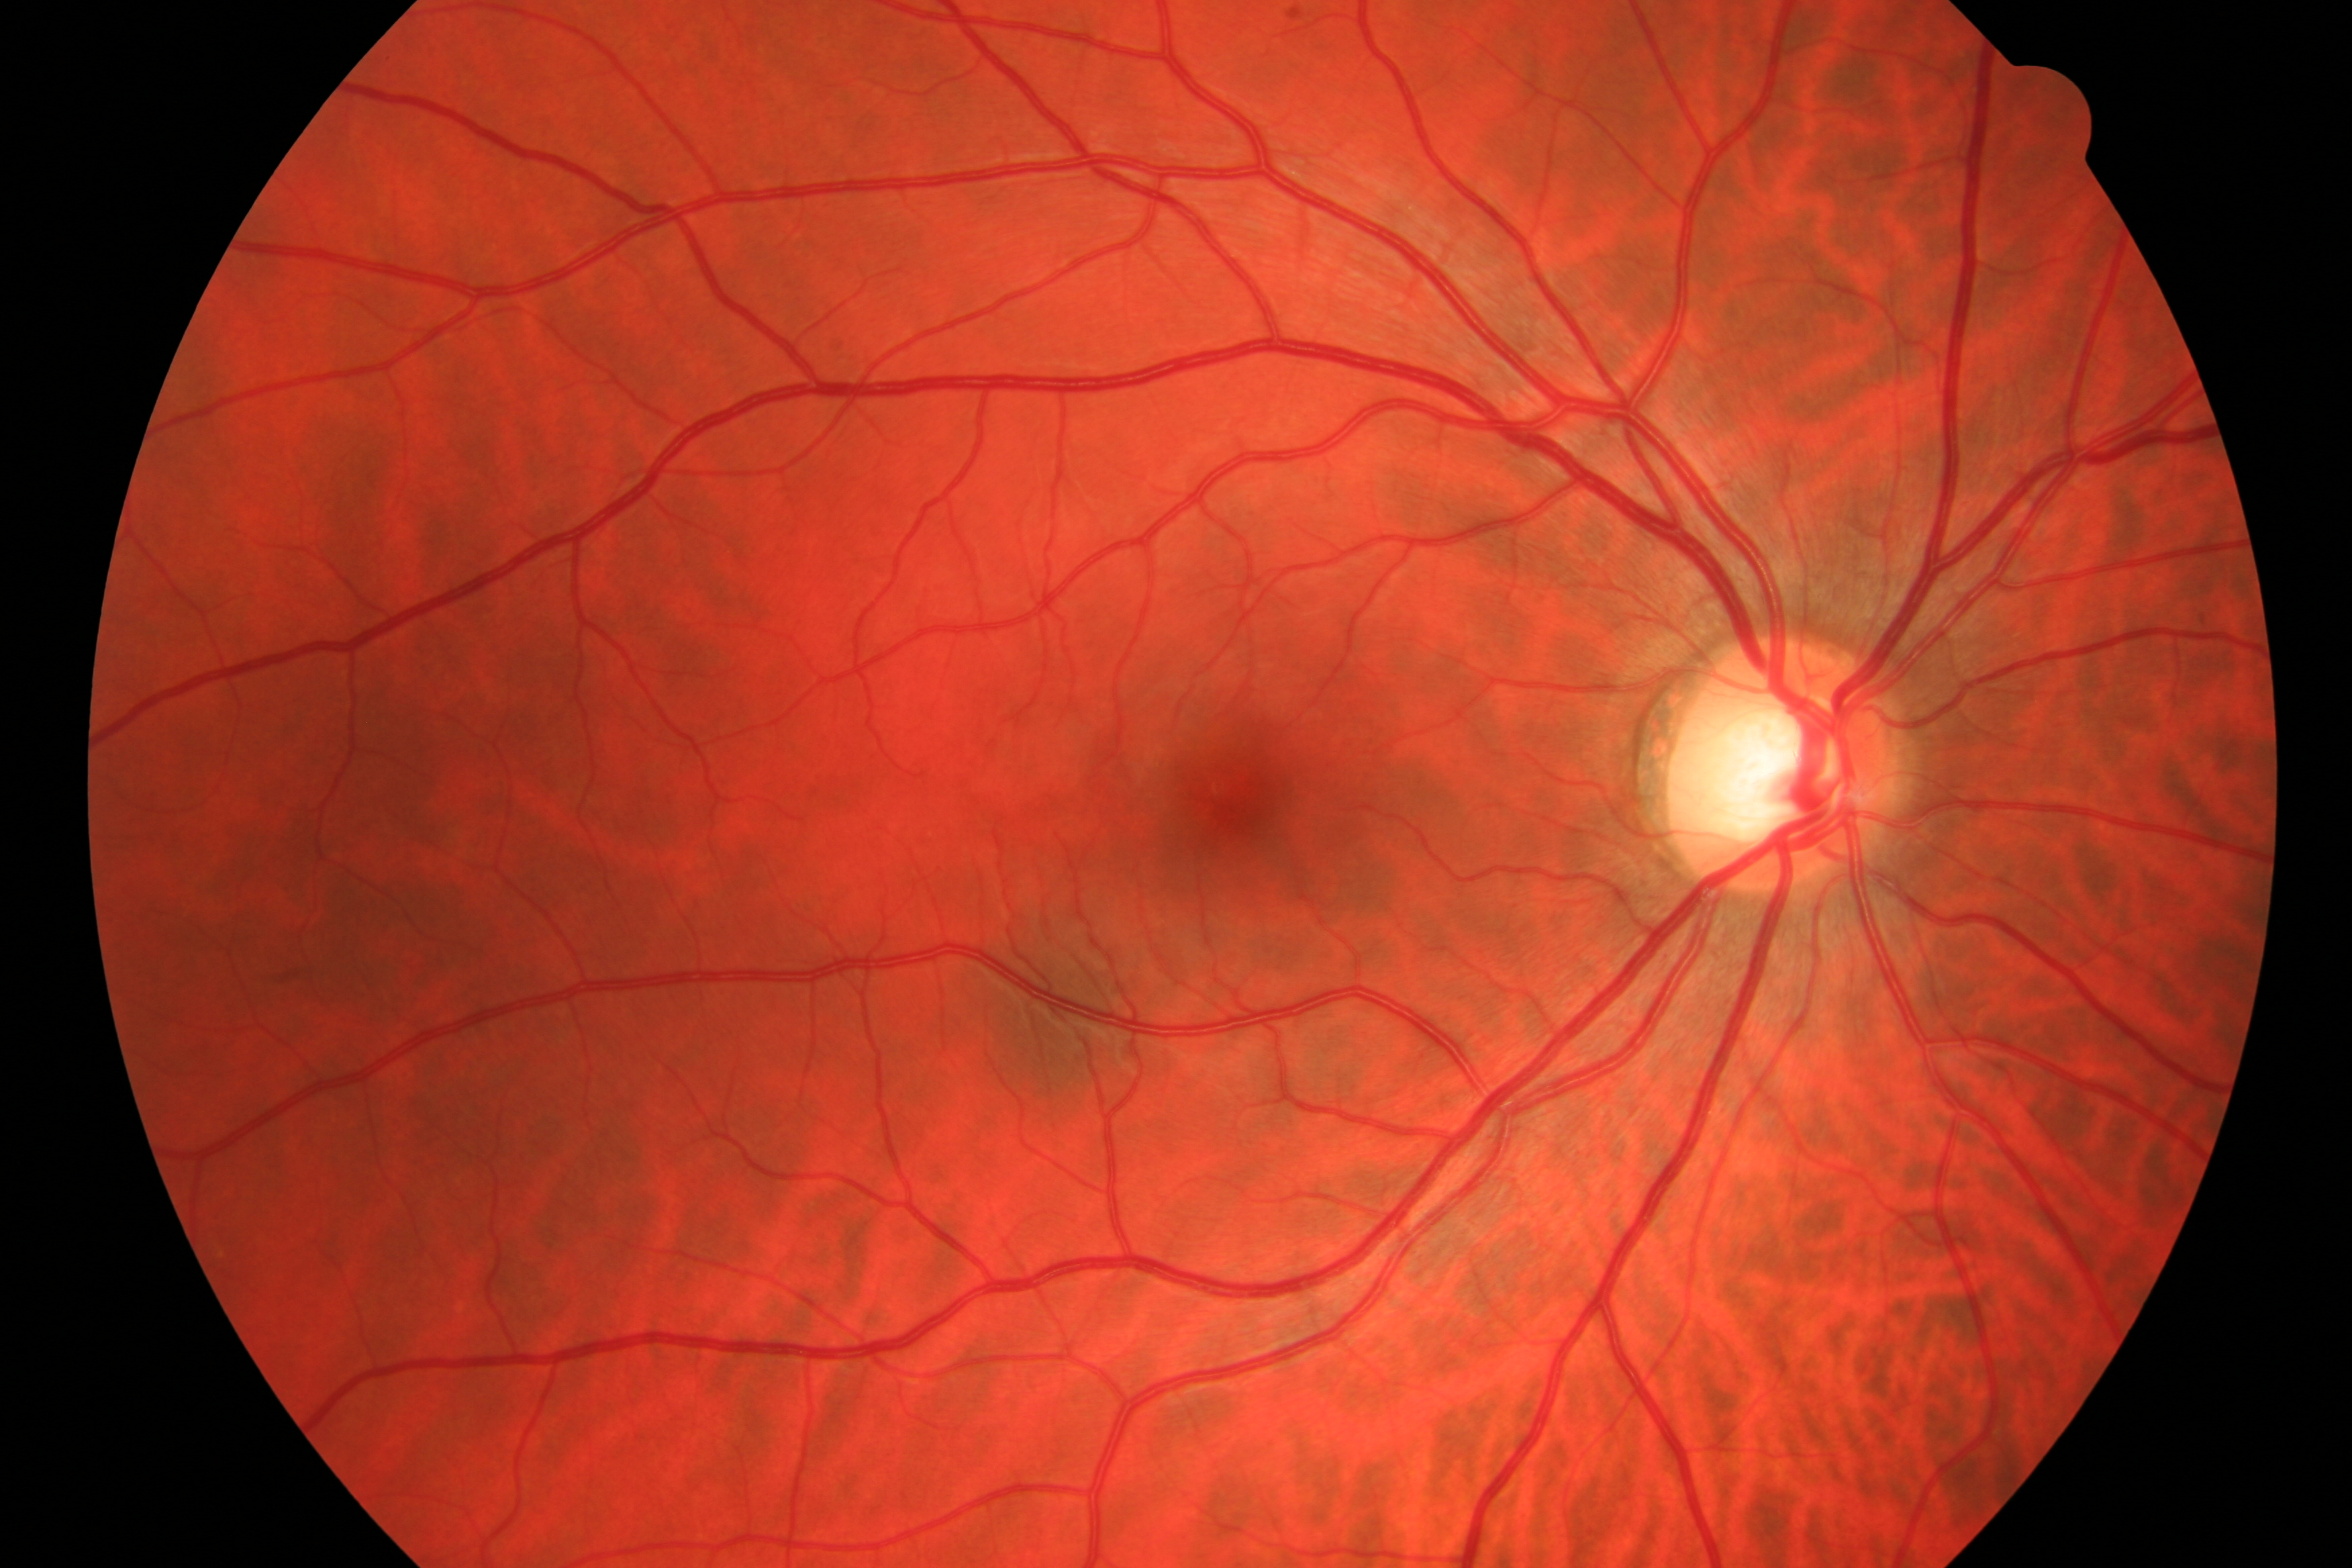
\includegraphics[width=0.3\textwidth]{01_h.jpg} \label{fig:sana}}
    \caption{Im\'agenes del dataset HRF. De izquierda a derecha: Retinopat\'ia  diabetica; Glaucoma; Imagen Sana}
		\label{fig:transferOverfeat}
\end{figure}

ARIA es una base de datos creada en 2006, en una colaboración de investigación entre  St. Paul's Eye Unit, Royal Liverpool University Hospital Trust, Liverpool, Reino Unido y el Departamento de Oftalmología, Ciencias Clínicas, Universidad de Liverpool, Liverpool, Reino Unido \cite{}. La base de datos consta de tres grupos; uno tiene 92 im\'agenes con degeneraci\'on macular relacionada con la edad, el segundo grupo tiene 59 im\'agenes con diabetes y un grupo de control se compone de 61 im\'agenes. El rastro de los vasos sangu\'ineos, la ubicaci\'on del disco \'optico y la f\'ovea est\'a marcada por dos expertos en an\'alisis de imagen como patr\'on de referencia. Las im\'agenes se capturan a una resoluci\'on de 768 {x} 576 p\'ixeles de colores RGB con 8 bits por plano de color con una c\'amara de fondo Zeiss FF450 con un campo de visi\'on de $50^{\circ}$ y se almacenan como archivos TIFF sin comprimir.\cite{fraz2012blood} \\ 

\begin{figure}[H]
\centering
\graphicspath {Figures} 
	  \label{fig:color}}
		\subfloat{\includegraphics[width=0.3\textwidth]{a_01.png} \label{fig:a_}}
		\subfloat{\includegraphics[width=0.3\textwidth]{c_1_7.png} \label{fig:c_}}
		\subfloat{\includegraphics[width=0.3\textwidth]{d_1_19.png} \label{fig:d_}}
    \caption{Im\'agenes del dataset ARIA. De izquierda a derecha: a; c; d}
		\label{fig:transferOverfeat}
\end{figure}

%-----------------------------------
%	SECTION 2
%-----------------------------------
\section{M\'etricas de calidad utilizadas}

En la Teor\'ia de detecci\'on de señales una curva ROC (Receiver Operating Characteristic, o Caracter\'istica Operativa del Receptor) es una representaci\'on gr\'afica de la sensibilidad frente al resultado de realizar 1 menos la especificidad, para un sistema clasificador binario seg\'un se var\'ia el umbral de discriminaci\'on. Otra interpretaci\'on de este gr\'afico es la representaci\'on de la raz\'on de verdaderos positivos frente a la raz\'on de falsos positivos tambi\'en seg\'un se var\'ia el umbral de discriminaci\'on (valor a partir del cual decidimos que un caso es un positivo).
Si aplicamos estos t\'erminos a este trabajo, la raz\'on de verdaderos positivos, se presenta cuando se pretende detectar y segmentar los vasos sangu\'ineos de la retina. El valor de verdaderos positivos estar\'a dada por la probabilidad que define la pertenencia de un p\'ixel a un vaso sanguineo. Del mismo modo un falso positivo, se define como la razon de que un p\'ixel no forma parte de un vaso sangu\'ineo, y esta determinaci\'on es correcta. Del mismo modo podemos definir lo que es un falso negativo y un verdadero negativo, cuyo significado es contrario a lo anterior. Es decir, un falso negativo es cuando se decide que un pixel no es parte de un vaso sangu\'ineo y en realidad si lo es, y un verdadero negativo es cuando se decide que un pixel es parte de un vaso sangu\'ineo, y no es as\'i en realidad. 
El an\'alisis de la curva ROC proporciona herramientas para seleccionar los modelos posiblemente \'optimos y descartar modelos sub\'optimos independientemente del coste de la distribuci\'on de las dos clases sobre las que se decide. Recientemente ha encontrado aplicaci\'on en \'areas como aprendizaje autom\'atico (o machine learning en ingl\'es), y miner\'ia de datos (data mining en ingl\'es).
Para dibujar una curva ROC s\'olo son necesarias las razones de Verdaderos Positivos (VPR) y de falsos positivos (FPR). La VPR mide hasta qu\'e punto un clasificador o prueba diagn\'ostica es capaz de detectar o clasificar los casos positivos correctamente, de entre todos los casos positivos disponibles durante la prueba. La FPR define cu\'antos resultados positivos son incorrectos de entre todos los casos negativos disponibles durante la prueba.
Una curva ROC se define por FPR y VPR como ejes x e y respectivamente, y representa los intercambios entre verdaderos positivos y falsos positivos. \cite{fawcett2004roc} \\
El mejor m\'etodo posible de segmentaci\'on se situar\'ia en un punto en la esquina superior izquierda, o coordenada (0,1) del espacio ROC, representando un 100\% de sensibilidad (ning\'un falso negativo) y un 100\% tambi\'en de especificidad (ning\'un falso positivo). A este punto (0,1) tambi\'en se le llama una clasificaci\'on perfecta. Por el contrario, una clasificaci\'on totalmente aleatoria dar\'ia un punto a lo largo de la l\'inea diagonal, que se llama tambi\'en l\'inea de no-discriminaci\'on, desde el extremo inferior izquierdo hasta la esquina superior derecha (independientemente de los tipos de bases positivas y negativas). El par\'ametro para evaluar la correctitud de la prueba, es el \'area bajo la curva que tomar\'a valores entre los valores m\'aximos y m\'inimos mencionados, es decir: 1  para un prueba perfecta y 0,5 si la prueba fue in\'util. 
\cite{wiki:curvaROC}.

\begin{figure}[H]
	{
	\centering
	\includegraphics[width=0.75\textwidth]{Figures/CurvaROC}
	\caption[Curva ROC]{Composici\'on de la curva ROC}
	\label{fig:Composici\'on de la curva ROC}
	}
\end{figure}


%-----------------------------------
%	SECTION 3
%-----------------------------------

\section{Resultados obtenidos durante el dise\'no del algoritmo}

%----------------------------------------------------------------------------------------
%	SECTION 4
%----------------------------------------------------------------------------------------

\subsection{Preprocesamiento}
\begin{itemize}
\item Extracci\'on de fondo: El objetivo de esta etapa consiste en suavizar la im\'agen, para esto calculamos el fondo de la misma, luego  restamos a la im\'agen original este fondo y de esta manera podemos remover el efecto de bias causado por la modalidad de captura de la im\'agen. Finalmente se convierte la im\'agen a double para tener mayor precisi\'on en las pr\'oximas etapas.
	\begin{itemize}
		\item Filtro de Mediana: para el calculo del filtro de mediana, se busc\'o cual era la mejor ventana a utilizar para cada uno de los dataset nombrados anteriormente, basandonos en el valor obtenido por la funci\'on vlroc de Matlab que determina el \'area bajo la curva promedio para cada set de im\'agenes. Los resultados arrojaron diferentes valores para cada conjunto de im\'agenes, por un lado se obtuvo un valor de ventana igual a 113 para el dataset HRF, lo cual es razonable para el tama\'no de dichas im\'agenes. Con este valor de ventana se obtuvo un \'area promedio de 0.93549792847311808; Por otro lado, con el conjunto de DRIVE se determin\'o que el mejor valor de ventana es 29, dando un valor de \'area bajo la curva de 0.89402376839923237,  lo cual tambi\'en es razonable ya que este tipo de im\'agenes son de menor tama\~no que las anteriores. Finalmente las im\'agenes ARIA resultaron un valor de ventana igual a 41 con un valor de \'area bajo la curva de 0.87129918114207383.
		
\begin{figure}[H]
\centering
\graphicspath {Figures} 
	  \label{fig:color}}
		\subfloat{\includegraphics[width=0.5\textwidth]{area_mediana_hrf} \label{fig:mediana_hrf}}
		\subfloat{\includegraphics[width=0.5\textwidth]{area_mediana_drive} \label{fig:mediana_drive}}
		\subfloat{\includegraphics[width=1\textwidth]{area_mediana_aria} \label{fig:mediana_aria}}
    \caption{\'Areas promedio para cada tam\~no de ventana. De izquierda a derecha: HRF; DRIVE; ARIA}
		\label{fig:transferOverfeat}
\end{figure}
		\item Filtro Gaussiano: para el calculo de \'area bajo la curva de este filtro, se utilizaron los par\'ametros por defecto del filtro, observ\'andose que los valores obtenidos, fueron muy por debajo de los obtenidos en los otros filtros, citando como  ejemplo que el mejor valor de \'area obtenido fue de 0.6581, dando finalmente un \'area promedio de  0,570545455. Por tal raz\'on se determin\'o que no es un filtro aplicable a este tipo de im\'agenes ya que no genera resultados buenos. 

\begin{figure}[H]
\centering
\graphicspath {Figures} 
	  \label{fig:color}}
		\subfloat{\includegraphics[width=1\textwidth]{area_gaussiano_aria} \label{fig:gaussiano_aria}}
    \caption{\'Area para cada im\'agen del dataset ARIA}
		\label{fig:transferOverfeat}
\end{figure}		
		
		\item Filtro Promedio: para el calculo del filtro promedio, se busc\'o cual era la mejor ventana a utilizar para cada uno de los dataset nombrados anteriormente, basandonos en el valor obtenido por la funci\'on vlroc de Matlab que determina el \'area bajo la curva promedio para cada set de im\'agenes. Los resultados arrojaron diferentes valores para cada conjunto de im\'agenes, por un lado se obtuvo un valor de ventana igual a 85 para el dataset HRF, lo cual es razonable para el tama\'no de dichas im\'agenes. Con este valor de ventana se obtuvo un \'area promedio de 0.91206707786006846. Por otro lado, con el conjunto de DRIVE se determin\'o que el mejor valor de ventana es 25, dando un valor de \'area bajo la curva de 0.86215776453164372,  lo cual tambi\'en es razonable ya que este tipo de im\'agenes es de menor tama\~no que las anteriores. Finalmente las im\'agenes ARIA resultaron un valor de ventana igual a 39 con un valor de \'area bajo la curva de 0.78861591936804754. 
		
\begin{figure}[H]
\centering
\graphicspath {Figures} 
	  \label{fig:color}}
		\subfloat{\includegraphics[width=0.5\textwidth]{area_media_hrf} \label{fig:mediana_hrf}}
		\subfloat{\includegraphics[width=0.5\textwidth]{area_media_drive} \label{fig:mediana_drive}}
		\subfloat{\includegraphics[width=1\textwidth]{area_media_aria} \label{fig:mediana_aria}}
    \caption{\'Areas promedio para cada tam\~no de ventana. De izquierda a derecha: HRF; DRIVE; ARIA}
		\label{fig:transferOverfeat}
\end{figure}
\end{itemize}
\item Extracci\'on de ruido: el objetivo de esta etapa consiste en disminuir el ruido de las im\'agenes que se genera en la captura de fondo de ojo, el cual puede ser generado por el dispositivo de captura utilizado. 
	\begin{itemize}
		\item Filtro anisotr\'opico: en este filtro se busc\'o el valor de la mejor iteraci\'on para cada set de im\'agenes. Los resultados obtenidos para cada set de im\'agenes fueron los siguientes. En el dataset HRF se obtuvo que la mejor iteraci\'on tiene un valor de 16, dando por resultado un \área de 0.93545909045136177. El dataset DRIVE tiene un valor de iteraci\'on para este filtro de 4 y un area de 0.8608094146529679 cuando se aplica con valor de media encontrado anteriormente y un valor de 5 cuando se aplica con el valor de mediana, dando un \'area de 0.90323495204661008. En el dataset ARIA el valor de la mejor iteraci\'on es 8 con un valor de area de 0.88453280013285718.

\begin{figure}[H]
\centering
\graphicspath {Figures} 
	  \label{fig:color}}
		\subfloat{\includegraphics[width=0.5\textwidth]{itera_anisotropica_hrf} \label{fig:anisotropica_hrf}}
		\subfloat{\includegraphics[width=0.5\textwidth]{itera_anisotropica_drive} \label{fig:mediana_drive}}
		\subfloat{\includegraphics[width=1\textwidth]{itera_anisotropica_aria} \label{fig:mediana_aria}}
    \caption{\'Areas promedio para el filtro anisotr\'opico. De izquierda a derecha: HRF; DRIVE; ARIA}
		\label{fig:transferOverfeat}
\end{figure}   
		\item Filtro de coherencia: para este filtro se realiz\'o una b\'usqueda para determinar cu\'al es la iteraci\'on que da el mejor valor de \'area bajo la curva. Para esto se realizaron iteraciones desde 1 hasta 130 en cada conjunto de im\'agenes. Los resultados obtenidos fueron analizados en funci\'on del tiempo computacional que tarda el algoritmo en procesar el conjunto de im\'agenes y el valor de \'area bajo la curva. El n\'umero de iteraciones en el dataset DRIVE que oobtuvo mejor resultado fue la iteraci\'on 75, donde la par\'abola llega al punto m\'aximo dando un \'area de 0.91120933863902276. En el caso del dataset HRF y ARIA, los resultados obtenidos por el filtro de coherencia fueron determinados en base al trade-off planteado antes. En ambos casos, el algoritmo no gener\'o una par\'abola como en el caso de DRIVE, sino que el valor del \'area creci\'o en todo momento. Finalmente se decidi\'o en base que el mejor valor de iteraci\'on quedar\'ia en 50 ya que el tiempo computacional que tarda el algoritmo en iterar hasta 130 en relaci\'on al resultado obtenido no es satisfactorio ya que la variaci\'on en el resultado se ve reci\'en en el tercer d\'igito decimal. El \'area bajo la curva en el dataset HRF con 50 iteraciones es 0.943776025051246 y un tiempo aproximado de 5 horas, mientras que para 130 iteraciones obtenemos un valor de \'area bajo  la curva de 0.94819116836674155 a un tiempo aproximado de 24 horas. Debido a que la relacion tiempo-ganancia es muy grande, se determin\'o que la mejor iteraci\'on en este conjunto de im\'agenes es 50.

\begin{figure}[H]
\centering
\graphicspath {Figures} 
	  \label{fig:color}}
		\subfloat{\includegraphics[width=0.5\textwidth]{itera_anisotropica_hrf} \label{fig:anisotropica_hrf}}
		\subfloat{\includegraphics[width=0.5\textwidth]{itera_anisotropica_drive} \label{fig:mediana_drive}}
		\subfloat{\includegraphics[width=1\textwidth]{itera_anisotropica_aria} \label{fig:mediana_aria}}
    \caption{NO SON LAS IMAGENES QUE VAN. De izquierda a derecha: HRF; DRIVE; ARIA}
		\label{fig:transferOverfeat}
\end{figure}  
		
	\end{itemize}
\end{itemize}


Los resultados obtenidos en los diferentes pipeline se muestran a continuaci\'on.


\begin{table}[H]
\begin{center}
\begin{tabular}{|l|l|l|l|}
\hline
Pipeline & \'Area HRF & \'Area DRIVE & \'Area ARIA \\
\hline \hline
1 & 0.943776025051246 & 0.17466860201317333 & 0.864926317715817 \\ \hline
2 & 0.17466860201317333 & 0.21162654260222666 & 0.3203105756103905 \\ \hline
3 & 0.93599954357138937 & 0.89698004054930147 & 0.87376408859019272 \\ \hline
4 & 0.94664138888216243 & 0.92281496665852036 & 0.88479933279751022 \\ \hline
\end{tabular}
\caption{\'Areas bajo la curva obtenidas en cada pipeline.}
\label{tabla:sencilla}
\end{center}
\end{table}
 

\begin{figure} [H] 
    \centering
    \begin{subfigure}[b]{0.3\textwidth}
        \includegraphics[width=\textwidth]{Figures/DRIVE/DRIVE_Pip1_21_training_cropped}
        \caption{Imagen preprocesada con el Pipeline 1}
        \label{fig:gull}
    \end{subfigure}
    ~ %add desired spacing between images, e. g. ~, \quad, \qquad, \hfill etc. 
      %(or a blank line to force the subfigure onto a new line)
    \begin{subfigure}[b]{0.3\textwidth}
        \includegraphics[width=\textwidth]{Figures/DRIVE/DRIVE_Pip3_21_training_cropped}
        \caption{Imagen preprocesada con el Pipeline 3}
        \label{fig:tiger}
    \end{subfigure}
    ~ %add desired spacing between images, e. g. ~, \quad, \qquad, \hfill etc. 
    %(or a blank line to force the subfigure onto a new line)
    \begin{subfigure}[b]{0.3\textwidth}
        \includegraphics[width=\textwidth]{Figures/DRIVE/DRIVE_Pip4_21_training_cropped}
        \caption{Imagen preprocesada con el pipeline 4}
        \label{fig:mouse}
    \end{subfigure}
    \caption{Resultados obtenidos luego del preprocesada para el dataset DRIVE}\label{fig:animals}
\end{figure}

\begin{figure} [H] 
    \centering
    \begin{subfigure}[b]{0.3\textwidth}
        \includegraphics[width=\textwidth]{Figures/HRF/HRF_Pip1_01_dr_cropped}
        \caption{Imagen preprocesada con el Pipeline 1}
        \label{fig:gull}
    \end{subfigure}
    ~ %add desired spacing between images, e. g. ~, \quad, \qquad, \hfill etc. 
      %(or a blank line to force the subfigure onto a new line)
    \begin{subfigure}[b]{0.3\textwidth}
        \includegraphics[width=\textwidth]{Figures/HRF/HRF_Pip3_01_dr_cropped}
        \caption{Imagen preprocesada con el Pipeline 3}
        \label{fig:tiger}
    \end{subfigure}
    ~ %add desired spacing between images, e. g. ~, \quad, \qquad, \hfill etc. 
    %(or a blank line to force the subfigure onto a new line)
    \begin{subfigure}[b]{0.3\textwidth}
        \includegraphics[width=\textwidth]{Figures/HRF/HRF_Pip4_01_dr_cropped}
        \caption{Imagen preprocesada con el pipeline 4}
        \label{fig:mouse}
    \end{subfigure}
    \caption{Resultados obtenidos luego del preprocesada para el dataset HRF}\label{fig:animals}
\end{figure}

\begin{figure} [H] 
    \centering
    \begin{subfigure}[b]{0.3\textwidth}
        \includegraphics[width=\textwidth]{Figures/ARIA/pipe1-aria_c_39_a_10_cropped}
        \caption{Imagen preprocesada con el Pipeline 1}
        \label{fig:gull}
    \end{subfigure}
    ~ %add desired spacing between images, e. g. ~, \quad, \qquad, \hfill etc. 
      %(or a blank line to force the subfigure onto a new line)
    \begin{subfigure}[b]{0.3\textwidth}
        \includegraphics[width=\textwidth]{Figures/ARIA/pipe3-aria_c_39_a_10_cropped}
        \caption{Imagen preprocesada con el Pipeline 3}
        \label{fig:tiger}
    \end{subfigure}
    ~ %add desired spacing between images, e. g. ~, \quad, \qquad, \hfill etc. 
    %(or a blank line to force the subfigure onto a new line)
    \begin{subfigure}[b]{0.3\textwidth}
        \includegraphics[width=\textwidth]{Figures/ARIA/pipe4-aria_c_39_a_10_cropped}
        \caption{Imagen preprocesada con el pipeline 4}
        \label{fig:mouse}
    \end{subfigure}
    \caption{Resultados obtenidos luego del preprocesada para el dataset ARIA}\label{fig:animals}
\end{figure}
%----------------------------------------------------------------------------------------
%	SUBSECTION 5
%----------------------------------------------------------------------------------------

\subsection{Extracci\'on de caracter\'isticas}


%----------------------------------------------------------------------------------------
%	SECTION 5
%----------------------------------------------------------------------------------------

\subsection{Entrenamiento y clasificaci\'on}

\section{Resultado del algoritmo de segmentaci\'on propuesto}

\section{Discusi\'on}

 
% Chapter Template

\chapter{Conclusiones} % Main chapter title

\label{Chapter5} % Change X to a consecutive number; for referencing this chapter elsewhere, use \ref{ChapterX}

%----------------------------------------------------------------------------------------
%	SECTION 1
%----------------------------------------------------------------------------------------

\section{Main Section 1}

 

%----------------------------------------------------------------------------------------
%	THESIS CONTENT - APPENDICES
%----------------------------------------------------------------------------------------

\appendix % Cue to tell LaTeX that the following "chapters" are Appendices

% Include the appendices of the thesis as separate files from the Appendices folder
% Uncomment the lines as you write the Appendices

\input{Appendices/AppendixA}
%\input{Appendices/AppendixB}
%\input{Appendices/AppendixC}

%----------------------------------------------------------------------------------------
%	BIBLIOGRAPHY
%----------------------------------------------------------------------------------------

\printbibliography[heading=bibintoc]

%----------------------------------------------------------------------------------------

\end{document}  
